\chapter{Results and Discussion}
\label{chap:Results}
Since a large part of our bachelor task consisted of face image quality research, this chapter is of great importance. After conducting the experiments in Chapter \ref{chap:subjective}, we gathered large amount of data, which we had to process. This data will be presented in the form of statistical calculations, such as box plots, correlation graphs and standard deviation graphs. The main goal of the chapter is to tie together the results we achieved in the objective and subjective face quality assessment, discuss them and present an in-depth look into the performance of the FIQMs relative to our collected ground truth data.   

\section{Main Experiment}
The results we achieved are split into two sections. In this first section the results of the objective assessment and our first subjective experiment will be presented and discussed. Both assessment categories are based on the three datasets provided by Mobai, which were described in Chapter \ref{chap:subjective}. 
%Utfylle mer her senere om hvordan seksjonen er oppbygd.

\subsection{Objective Assessment Scores}
The FIQMs presented in Chapter \ref{chap:FQA} use different approaches to predict the perceived face quality. Their predicted perception of quality is supposed to correlate with human assessment, which is the whole purpose of the metrics. The objective predictions produced by the FIQMs were measured up to human assessment to evaluate how true to their purpose they were. This evaluation was carried out by comparing the results of the FIQMs against the results gathered from human observers. The same resized images used in our first subjective experiment were used as input to our two FIQMs. 
\newpage

\begin{figure}[h]
\centering
    \subfloat[Combined passport alike]
        {\includegraphics[scale = 0.36]{figures/ISO_FaceQnet1.png}\label{fig:combinedpassportalikeplot}}
    \subfloat[Capture from photo]
        {\includegraphics[scale = 0.36]{figures/ISO_FaceQnet2.png}\label{fig:capturefromphotoplot}}
    \subfloat[Selfie dataset]
        {\includegraphics[scale = 0.36]{figures/ISO_FaceQnet3.png}\label{fig:selfiedatasetplot}}
    \caption{2D correlation graphs of the scores provided by the FIQMs on the three datasets with ISO Metrics scores along the x-axis and FaceQnet scores along the y-axis. The Spearman and Pearson correlation coefficients, including the coefficient of determination, are calculated.}
    \label{fig:corrFIQMs}
\end{figure}

The three plots depicted in Figure \ref{fig:corrFIQMs} show the scores of each image, which are represented by dots, in the three datasets. One can easily see the large difference in scores predicted by the two FIQMs. In regards to the first plot, with the ``Combined passport alike'' dataset, ISO Metrics had a large gap between the ratings provided. Most of the images were given a score above 0.9, while some received the lowest score of zero. Images with a score of zero provided by ISO Metrics were usually of faces where both eyes were not visible. ISO Metrics is coded in such a way that facial images where both eyes are not visible will be filtered out and provided with a score of zero. FaceQnet however, rated the images far more evenly between the 0.2 and 0.6 range. Figure \ref{fig:capturefromphotoplot} shows far more evenly distributed scores even though the scores from FaceQnet were significantly lower than ISO Metrics. As for Figure \ref{fig:selfiedatasetplot} the scores from ISO Metrics were equally spread from zero to one, where as most of the FaceQnet scores were zero. The images rated zero were mostly because the cropping part of FaceQnet failed. The images were therefore manually provided a score of zero. In other words, FaceQnet is not a suitable FIQM for the Selfie-dataset.  

The sample Pearson correlation coefficient ($r$) was calculated as: 
\begin{equation}
    {\displaystyle r={\frac {\sum _{i=1}^{n}(x_{i}-{\bar {x}})(y_{i}-{\bar {y}})}{{\sqrt {\sum _{i=1}^{n}(x_{i}-{\bar {x}})^{2}}}{\sqrt {\sum _{i=1}^{n}(y_{i}-{\bar {y}})^{2}}}}}}
\end{equation}
where $n$ is the sample size, $x_{i}$ and $y_{i}$ denotes the individual sample points (scores) from ISO Metrics and FaceQnet respectively while ${\bar {x}}={\frac {1}{n}}\sum _{i=1}^{n}x_{i}$ and ${\bar {y}}={\frac {1}{n}}\sum _{i=1}^{n}y_{i}$ represents the sample means from both FIQMs. Another type of correlation coefficient, the Spearman rank correlation coefficient ($\rho$) \cite{wiki:spearman} was also calculated because it does not assume that both variables are normally distributed.

As for the plots depicted in Figure \ref{fig:corrFIQMs} one can see that a correlation between ISO Metrics and FaceQnet on the three datasets was near no existent. Figure \ref{fig:capturefromphotoplot} showed the closest to zero correlation between the datasets. The $\rho$ and $r$-values even show a negligible negative correlation which is confirmed by the red linear regression line which slightly points downwards. On the contrary Figure \ref{fig:capturefromphotoplot} showcases a $r$-value of 0.34 which is still considered a weak correlation, but is noticeably higher than the two other datasets. !!!The reasoning for this is because of the??? . The rightmost plot is similar to plot (a), but with a negligible positive correlation. It is highly likely that if FaceQnet had worked for the dataset, the correlation would be different. 


\subsection{Subjective Assessment Scores}
As earlier mentioned, the first subjective experiment was supposed to gather ground truth data about each of the three datasets provided by Mobai. These datasets were equally split and mixed amongst the three survey sessions. Since the survey sessions consisted of images from all datasets, the data gathered from each survey session had to be organized and matched with the images of the corresponding dataset. That way the ground truth data could be analyzed on the original datasets and not on the datasets used for each survey session.

\begin{figure}[h]
    \centering
    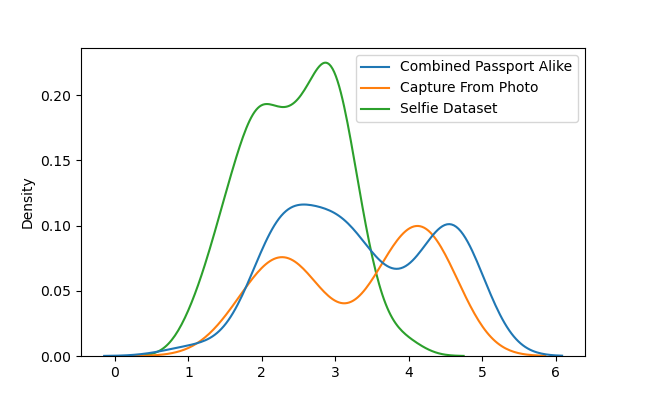
\includegraphics[width=0.7\textwidth]{figures/KernelPlots2.png}
    \caption{Kernel density estimation on the subjective scores between one and five on each dataset. There is a clear difference between the quality of the Selfie dataset vs the two others.}
    \label{fig:kerneldensity}
\end{figure}

We calculated the mean opinion score (MOS) on each image in the datasets and in Figure \ref{fig:kerneldensity} one can see how the subjective scores were distributed between the datasets. The quality of the images in the Selfie dataset were more consistent than the two other datasets, because it was more evenly distributed. The score distribution for Combined passport alike and Capture from photo were quite similar which was expected given that the images in the datasets were related. The standard deviation was calculated for every image, but also for each dataset and the datasets combined. The average standard deviation ($\overline{\sigma}$) for both experts and non-experts on all three datasets combined was calculated to $\overline{\sigma} = 0.7488$. This confirmed that the participants had an equal understanding of what defined a good or a bad image. Given that we were collecting ground truth data, it was expected that the deviation should be low.   

\newpage

\begin{figure}[h]
\centering
    \subfloat[Combined passport alike]
        {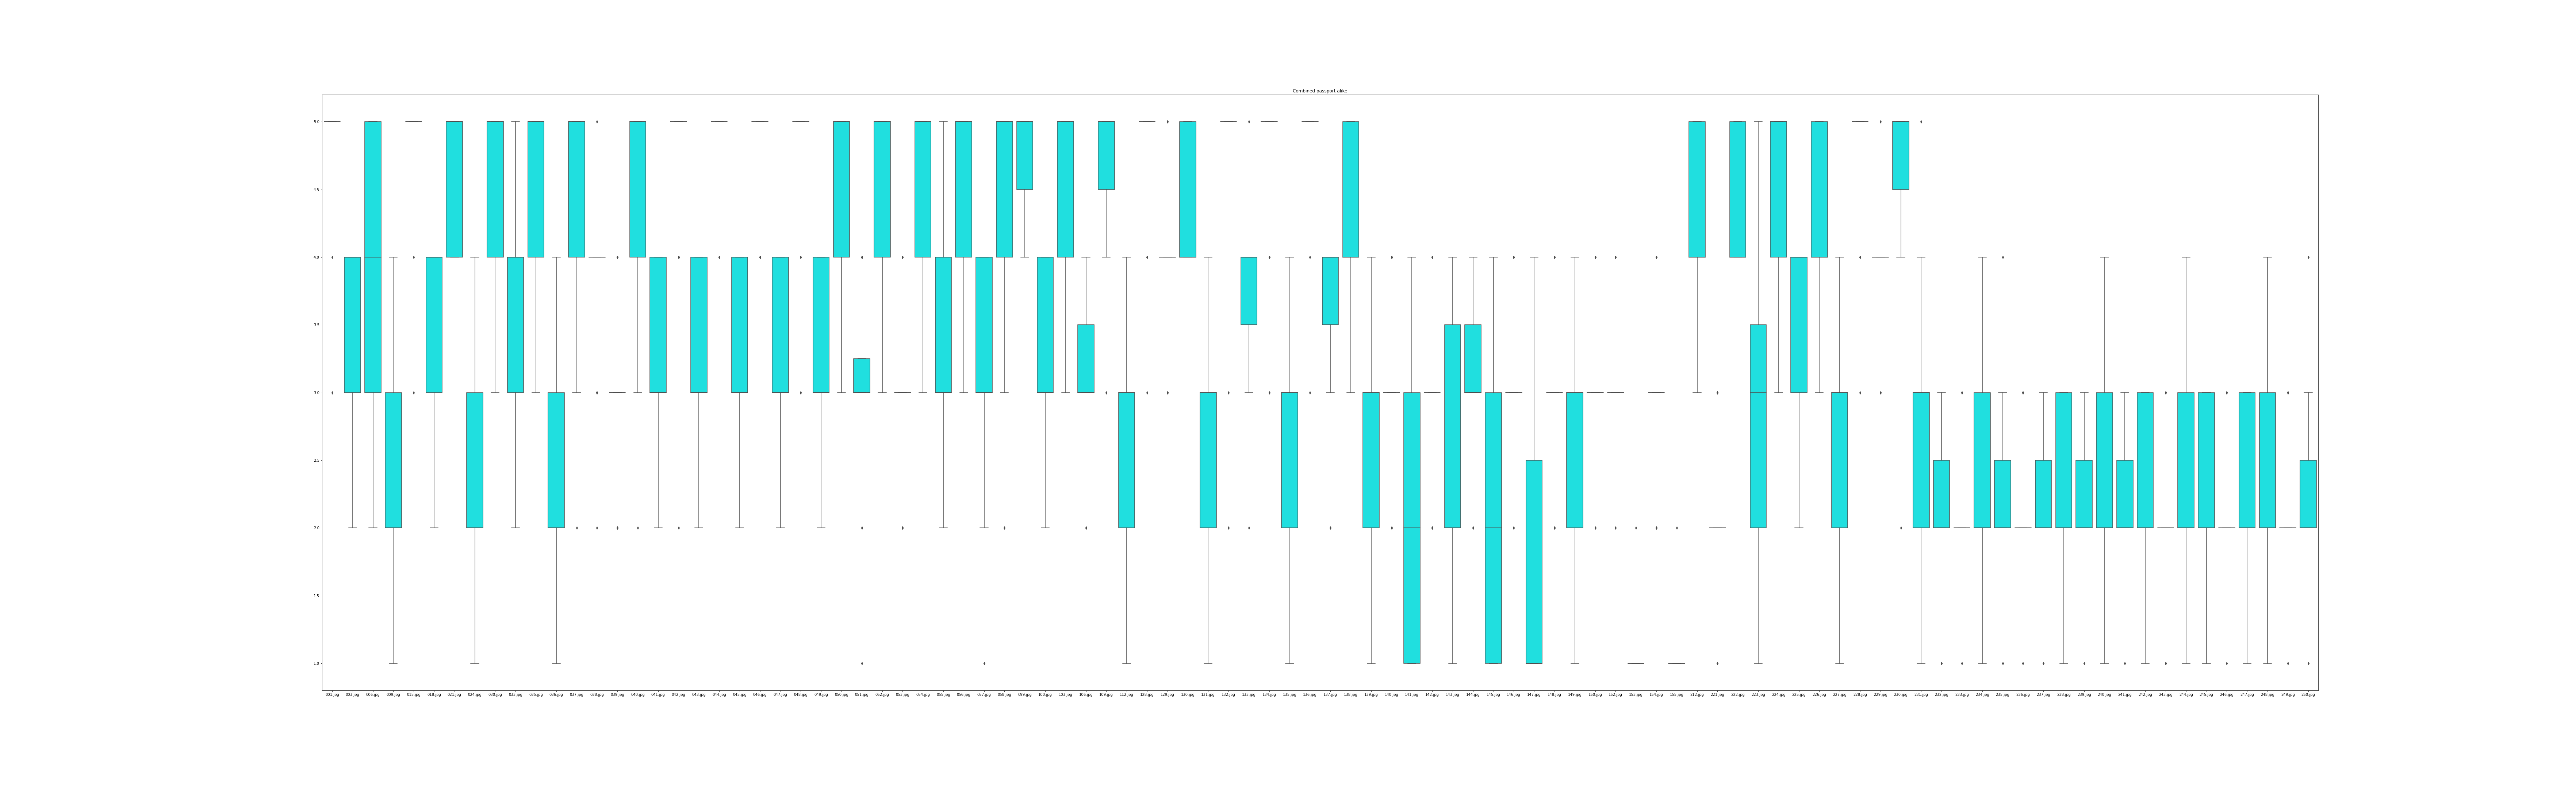
\includegraphics[width=1.0\textwidth]{figures/boxplot1.png}\label{fig:combinedpassportalikeboxplot}}
        \quad
    \subfloat[Capture from photo]
        {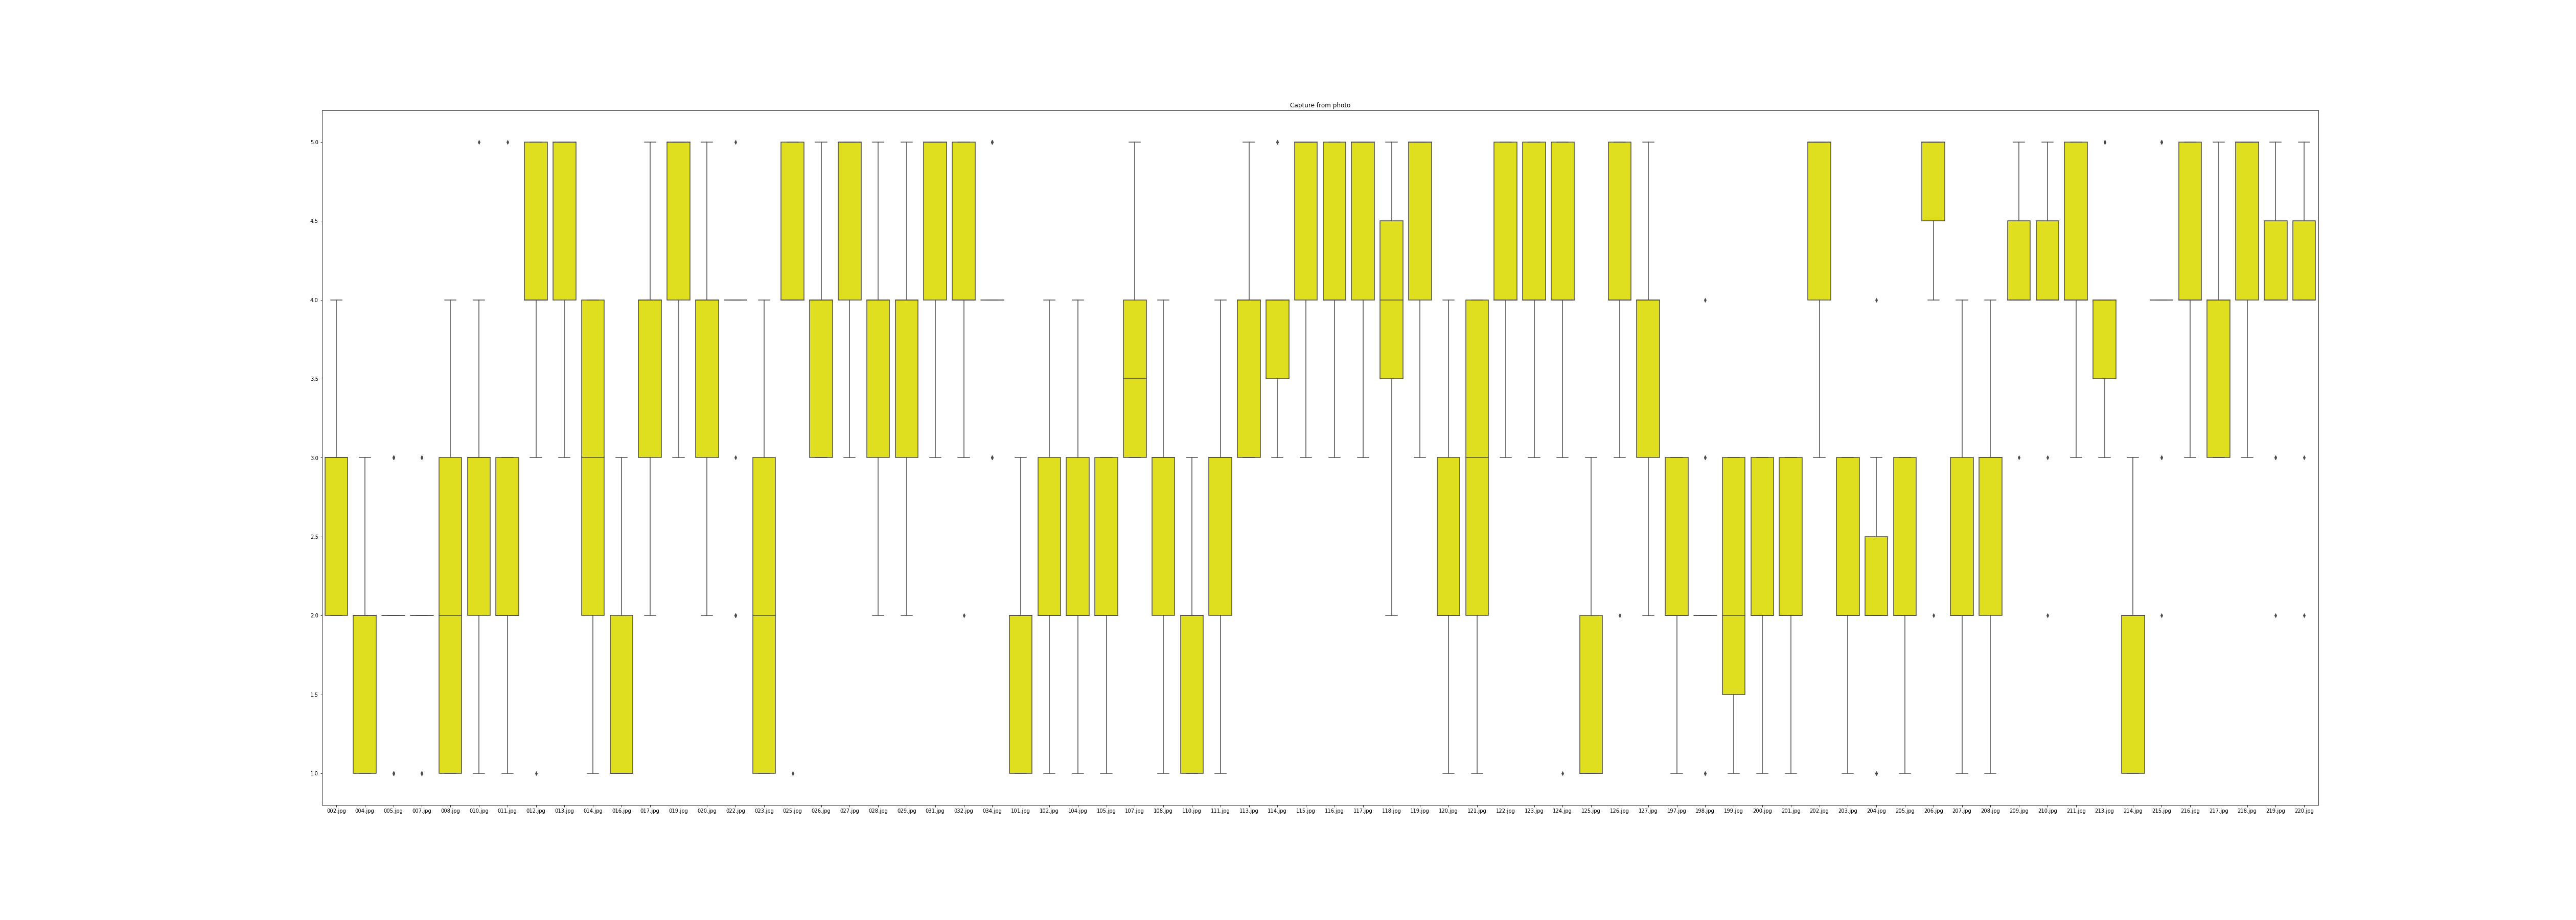
\includegraphics[width=1.0\textwidth]{figures/boxplot2.png}\label{fig:capturefromphotoboxplot}}
        \quad
    \subfloat[Selfie dataset]
        {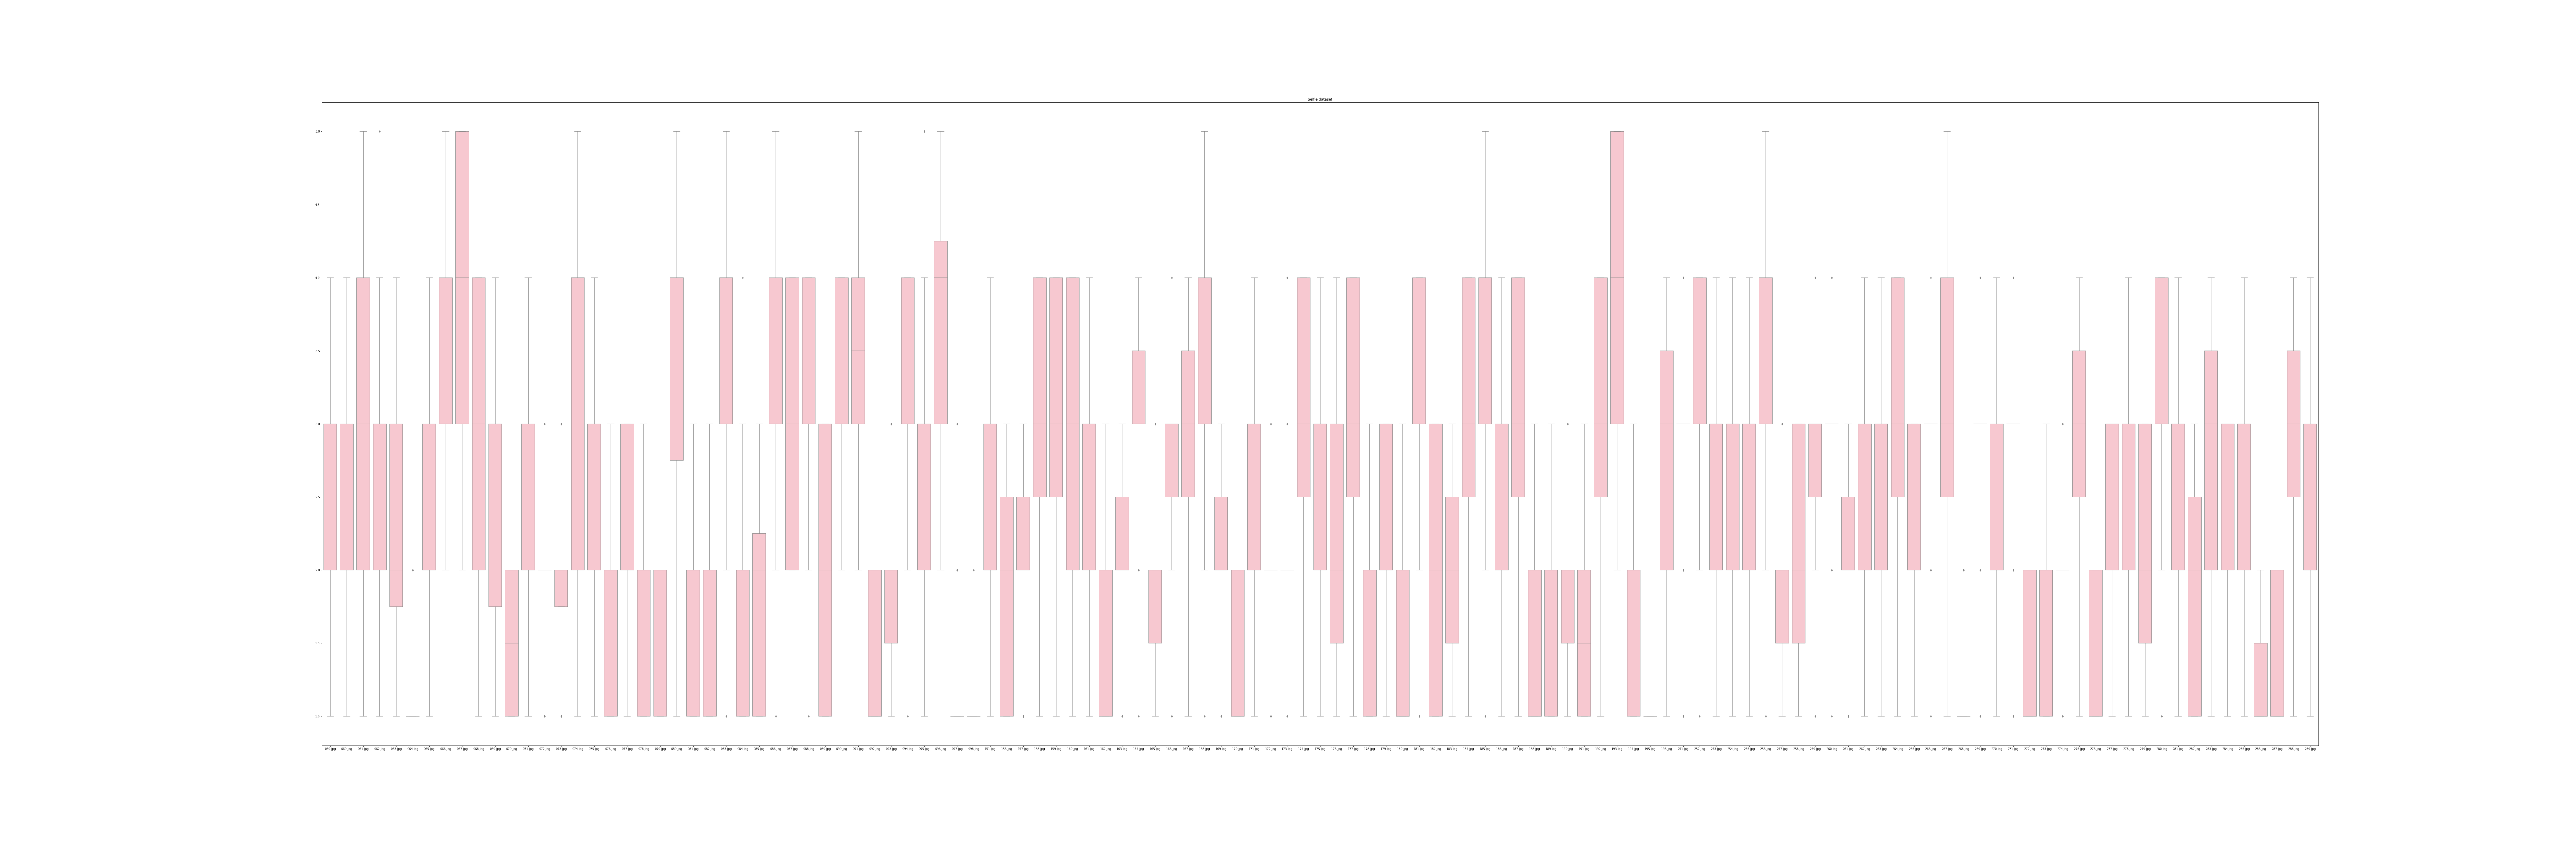
\includegraphics[width=1.0\textwidth]{figures/boxplot3.png}\label{fig:selfiedatasetboxplot}}
    \caption{Standard box plots of the images in the datasets. It shows the outliers, the min and max whiskers, the lower (Q1) and upper quartile (Q3) as well as the median (Q2) of the ground truth data produced by the survey participants.}
    \label{fig:boxplot}
\end{figure}

Figure \ref{fig:boxplot} depicts three box plots of the score distribution of each image in a dataset. The whiskers extending from either side show the extent of the data. Some of the images are shown as tiny lines with no body, which indicates that the majority agreed upon a similar score. This is especially apparent in the first plot which also generated the lowest standard deviation of $\sigma = 0.6707$. The two remaining datasets received a similar standard deviation of $\sigma = 0.7891$ and $\sigma = 0.7872$ respectively. Some images had greater variety than others. The selfie dataset contained some of those, but all in all the general participants rated images alike. Even between the experts and non-experts, the evaluation was more or less equal. In fact non-experts had a slightly better standard deviation of $\sigma = 0.6908$, than the experts of $\sigma = 0.7608$. 


\subsection{FIQMs vs Ground Truth Data}
The subjective scores had to be normalized in order to be compared with the objective scores. Our survey initially had a categorical judgment with a scale from one to five, which had to be converted to scores between zero and one. It is easy to think that the MOS for each image should be divided by the number of score alternatives in the subjective experiment, which in this case was five. However it is worth noting that had we only divided the subjective scores by five, the subjective scores would never fall below 0.2. This means that the FIQMs could provide scores from zero to one, while the ground truth data was from 0.2 to one. Dividing by five would therefore provide us with an uneven scoring scale where a score of five equals 100\% while the lowest score of one equals 20\% instead of 0\%. We needed a five-point scale that would increment the score alternatives with 25\% starting from 0\%. To properly convert a five-point scale to percentages we used the following equation on every image:

\begin{equation}
    MOS_{Normalized} = \frac{MOS_{} - 1}{4}
\end{equation}

\subsubsection{ISO Metrics}
\begin{figure}[h]
\centering
    \subfloat[Combined passport alike]
        {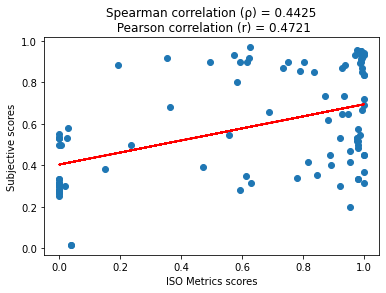
\includegraphics[scale = 0.36]{figures/ISO_Subjective1.png}\label{fig:iso_SUB1}}
    \subfloat[Capture from photo]
        {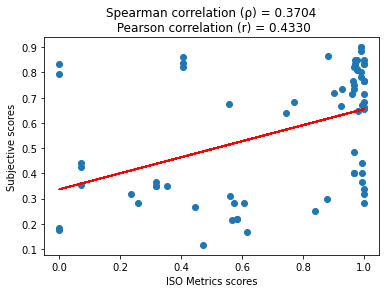
\includegraphics[scale = 0.36]{figures/ISO_Subjective2.png}\label{fig:iso_SUB2}}
    \subfloat[Selfie dataset]
        {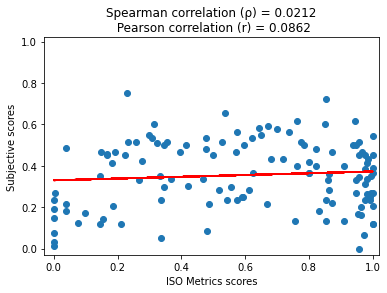
\includegraphics[scale = 0.36]{figures/ISO_Subjective3.png}\label{fig:iso_SUB3}}
    \caption{2D correlation graphs of the scores provided by the FIQMs on the three datasets with ISO Metrics scores along the x-axis and subjective ground truth data along the y-axis. The Spearman and Pearson correlation coefficients are calculated.}
    \label{fig:corrISOsvsSub}
\end{figure}
\noindent
The correlation between ISO Metrics and the subjective scores was considerably higher, although still low, than the correlation between ISO Metrics and FaceQnet for Combined passport alike and Capture from photo which is shown by the plots depicted in Figure \ref{fig:corrISOsvsSub}. The correlation coefficients were just shy of 0.5 which indicated a low to moderate association whereas the correlation on the selfie dataset was non existent. The performance of ISO Metrics was clearly worse on the Selfie dataset relative to the two others. The FIQM was challenged by the dataset which was not surprising given that the images were of mediocre face quality which ISO Metrics often tends to over evaluate. In other words ISO Metrics was not suited for the Selfie dataset.  

\subsubsection{FaceQnet}
\begin{figure}[h]
\centering
    \subfloat[Combined passport alike]
        {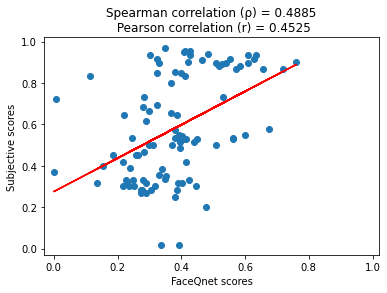
\includegraphics[scale = 0.36]{figures/FaceQNet_Subjective1.png}\label{fig:face_SUB1}}
    \subfloat[Capture from photo]
        {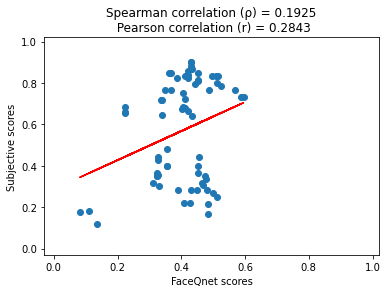
\includegraphics[scale = 0.36]{figures/FaceQNet_Subjective2.png}\label{fig:face_SUB2}}
    \subfloat[Selfie dataset]
        {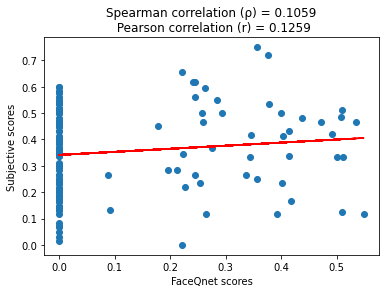
\includegraphics[scale = 0.36]{figures/FaceQNet_Subjective3.png}\label{fig:face_SUB3}}
    \caption{2D correlation graphs of the scores provided by the FIQMs on the three datasets with FaceQnet scores along the x-axis and subjective ground truth data along the y-axis. The Spearman and Pearson correlation coefficients are calculated.}
    \label{fig:corrFACEQNETsvsSub}
\end{figure}
\noindent
The correlation between FaceQnet and the ground truth data regressed with each dataset the same way as ISO Metrics and the ground truth data did. The performance of the two FIQMs was comparable on all the datasets. Combined passport alike achieved the highest correlation of the datasets, with Spearman and Pearson values similar to the ones in Figure \ref{fig:iso_SUB1}. Like ISO Metrics, the performance of FaceQnet on Capture from photo was worse than Combined passport alike, but this time FaceQnet performed slightly worse. The performance on the Selfie dataset was even worse with a non-existing correlation. 

\subsubsection{Combining the FIQMs}
An interesting though the team came by, was if the correlation between the FIQMs and the ground truth data significantly would be affected by combining the two quality scores predicted by the metrics. The new score for each image was calculated by adding and then dividing the scores of FaceQnet and ISO Metrics by two. This was tested only on Combined passport alike and Capture from photo. Since FaceQnet did not work for over 50\% of the images in the Selfie dataset, we found no reason to combine the two scores on that dataset. 

Figure \ref{fig:corrAVGvsSub} shows the correlation coefficients and the linear regression line calculated on the two datasets. The plot depicted in Figure \ref{fig:avg_SUB1} shows the highest correlation coefficients we ever achieved during our experiment. The $r$-value of 0.6045 and the $\rho$-value of 0.5942 were considerably higher than the correlation coefficients of the FIQMs individually. An value around 0.6 would indicate a moderate to strong correlation between the two data types. Even Capture from photo achieved an increased correlation. Initially ISO Metrics performed better on the dataset than FaceQnet, but after combining them, the combined scores performed slightly better than ISO Metrics. The correlation was still considered low to moderate. 
\begin{figure}[h]
\centering
    \subfloat[Combined passport alike]
        {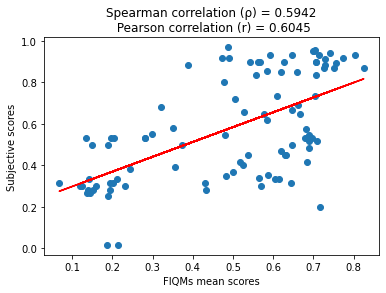
\includegraphics[scale = 0.4]{figures/FIQMAVGSubjective1.png}\label{fig:avg_SUB1}}
    \subfloat[Capture from photo]
        {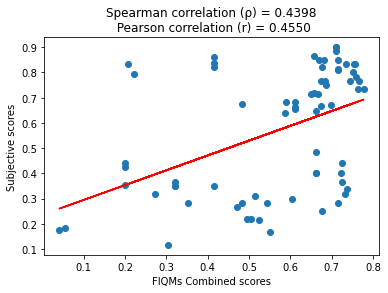
\includegraphics[scale = 0.4]{figures/FIQMAVGSubjective2.png}\label{fig:avg_SUB2}}
    \caption{2D correlation graphs of the average scores provided by the FIQMs on Combined passport alike and Capture from photo. The average FIQMs scores are displayed along the x-axis and subjective ground truth data along the y-axis. The Spearman and Pearson correlation coefficients are calculated.}
    \label{fig:corrAVGvsSub}
\end{figure}

\subsubsection{Error Method}
Plotting the results of the FIQMs against the ground truth data was not enough to assess the performance of the metrics on the datasets. Although the correlation coefficients on the datasets mostly were below 0.5 and indicated low to moderate correlation, error methods such as Root Mean Square Error (RMSE) can be used to track both the efficiency and accuracy of our metrics. The RMSE-values were calculated by the following general formula: 
\begin{equation}
    RMSE = \sqrt{\frac{1}{N}\sum _{i=1}^{N}(Predicted_{i} - Actual_{i})^2}
\end{equation}
$N$ equaled the number of samples, and in our case these were images. The predicted values denoted the objective scores by the FIQMs while the actual values were the corresponding ground truth data. This calculation gave us the standard deviation of the prediction errors. In other words, RMSE measured how far from the linear regression line the predicted values were. 
\newpage

\begin{table}[h]
\caption{The calculated RMSE values of the FIQMs on the datasets relative to the ground truth data. The RMSE value was not calculated for the Selfie dataset with the combined scores of the FIQMs. The `X' symbolises this.}
\resizebox{\textwidth}{!}{%
\begin{tabular}{|
>{\columncolor[HTML]{EFEFEF}}c |
>{\columncolor[HTML]{FFFFFF}}c |
>{\columncolor[HTML]{FFFFFF}}c |
>{\columncolor[HTML]{FFFFFF}}c |}
\hline
\multicolumn{1}{|c|}{\cellcolor[HTML]{C0C0C0}\textbf{RMSE-values}} &
  \multicolumn{1}{c|}{\cellcolor[HTML]{EFEFEF}ISO Metrics} &
  \cellcolor[HTML]{EFEFEF}FaceQnet &
  \multicolumn{1}{c|}{\cellcolor[HTML]{EFEFEF}FIQMs Combined} \\ \hline
Combined passport alike & 0.3675 & 0.3031 & 0.2262 \\ \hline
Capture from photo      & 0.3551 & 0.2887 & 0.2309 \\ \hline
Selfie dataset          & 0.4342 & 0.3253 & X \\ \hline
\end{tabular}%
}
\end{table}



\section{Second Experiment}
This second section is about the second subjective experiment we conducted based on our own dataset of 250 images. 
%Spider på rotert vs ikke rotert 
\subsection{Objective Assessment Scores}
\subsection{Subjective Assessment Scores}